\documentclass[11pt]{article}

\usepackage[a4paper, total={6in, 10in}]{geometry}
\usepackage{graphicx}
\usepackage{float}

\title{Is Florida getting warmer?}

\author{Tash Ramsden}

\date{}

\begin{document}
    \maketitle
    
    \section{Introduction}

    This Practical assumes you have at least a basic understanding of correlation coefficients and p-values.

    \begin{figure}[H]
        \centering
            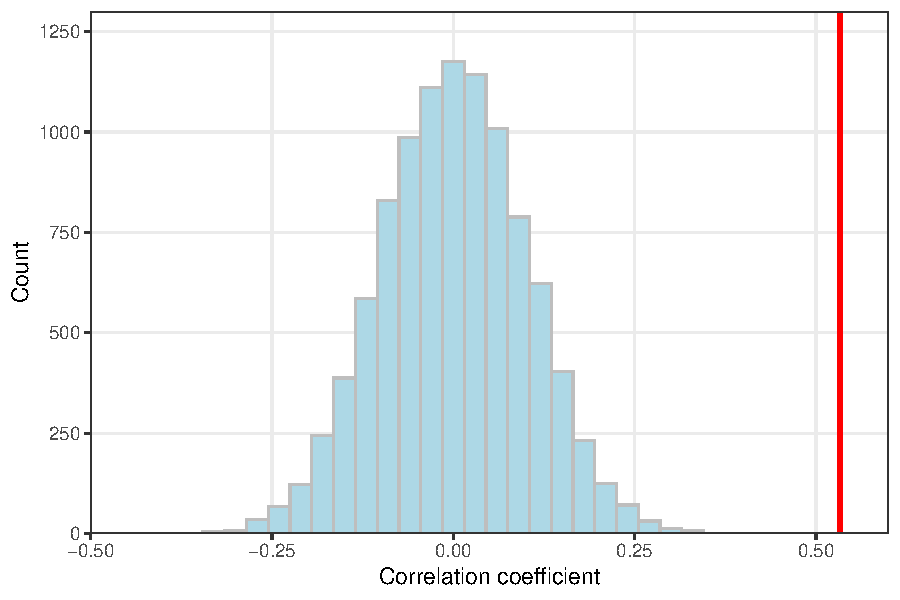
\includegraphics[width=0.7\linewidth]{coefs_hist.pdf}
            \caption{Histogram of correlation coefficients.}
            \label{fig:coefs_hist}
    \end{figure}

    Your goal is to write an R script that will help answer the question: Is Florida getting warmer? Call this script Florida.R.

    To answer the question, you need to calculate the correlation coefficients between temperature and time. However, you can’t use the standard p-value calculated for a correlation coefficient, because measurements of climatic variables in successive time-points in a time series (successive seconds, minutes, hours, months, years, etc.) are not independent. Therefore you will use a permutation analysis instead, by generating a distribution of random correlation coefficients and compare your observed coefficient with this random distribution.
    
\end{document}
